\chapter{ntsc pal}
\label{sec:ntsc_pal}
\lstset{style=68KStyle}

In the 1980s and 1990s games were played on cathode ray tube televisions. Like
with everything, there were competing standards. And like with everything, Americans
did things one way (NTSC) and Europe did things another (PAL). The rest of the world
got to choose which horse to back.

There are many technical differences between NTSC and PAL, but only one that Jeff Minter
really needed to worry about in \textit{Tempest 2000}: how many lines of pixels each
standard allowed. NTSC allowed a measly 241, while PAL televisions came with a princely 287.

Faced with releasing a video game that could be played on televisions in both America and Europe, 
the developer needed to figure out which of the two it was playing on and adjust the dimensions
of the screen it was writing to accordingly.

When launched one of the earliest tasks is to do this figuring out. Fortunately there was a 
magic number available from the Jaguar hardware that would tell it what was what. This magic
number lived at the hardware address register \icode{\$F14002}. Here we can see the \icode{VideoIni}
routine take care of this business, querying the register, setting some dimensions based on the
reading it gets, and most importantly for the rest of the game, setting a global variable called
\icode{pal} that can be used to perform any adhoc fiddling during gameplay to ensure a display
consistent with the player's ageing television hardware.

\begin{lstlisting}
VideoIni:
        movem.l d0-d6,-(sp)        ; Store d0-d6 in the stack.
        clr pal                    ; Clear the global pal variable
    
        move.w  BASE+$14002,d0     ; Check the JOY2(!) port.
        and.w   #$10,d0            ; Check if the magic bit is set..
        beq     ispal              ; .. if not, it's PAL so skip to ispal.
    
        ; Otherwise it's NTSC.
        move.w  #ntsc_hmid,d2      ; Set the Horizontal mid-point
        move.w  #ntsc_width,d0     ; Set the width.
        move.w  #ntsc_vmid,d6      ; Set the vertical mid-point.
        move.w  #ntsc_height,d4    ; Set the height.
    
        bra     doit               ; Actually apply the above values.
ispal:
        move.w  #pal_hmid,d2       ; Set the Horizontal mid-point
        move.w  #pal_width,d0      ; Set the width.
        move.w  #pal_vmid,d6       ; Set the vertical mid-point.
        move.w  #pal_height,d4     ; Set the height.
        move #1,pal                ; Set the global pal variable.
\end{lstlisting}

There are numerous places where this kind of fiddling will be necessary. Early on in the
game's launch sequence we will query this \icode{pal} setting to set various fix-up
variables that can be used to centre text and images depending on the height of the
screen:

\begin{lstlisting}
; *******************************************************************
; Set up the NTSC/PAL options.
; *******************************************************************
spall:
        btst.b #6,sysflags         ; Are controllers enabled?
        beq slopt
        move.l #o2s3,option2+16
slopt:
        clr palside
        clr paltop
        bclr.b #5,sysflags         ; Flag PAL as not enabled.
        tst pal
        beq notpal1
        ; Set screen adjustments for PAL
        move #6,palside
        move #10,paltop
        move #40,palfix1           ; Y centre fix for rectangles in PAL
        move #20,palfix2           ; Y centre fix for text in PAL
        move.l #$140000,palfix3    ; Y centre fix for PAL
        bset.b #5,sysflags         ; Set PAL as enabled.
notpal1: rts
\end{lstlisting}

Here's an example where we're going to display some text on the screen
("Press Option for Beastly Mode!") and need to figure out whether we're on
a PAL or NTSC screen to decide where to place the text so that it's vertically
centred.
\begin{lstlisting}
draw_oo:
        bsr draw_o                 ; Call the common draw_o rotuine first.
        btst.b #2,sysflags         ; Is Beastly Mode enabled?
        beq rrrts                  ; If so, return early.
        tst h2h                    ; Are we playing a head-to-head game?
        bne rrrts                  ; If so, return early.
        lea bstymsg,a0             ; "PRESS option FOR BEASTLY MODE!"
        lea cfont,a1               ; Load the small regular font to a1.
        move #180,d0               ; Set Y position of text.
        tst pal                    ; Are we on a PAL screen?
        beq gnopal2                ; If not, skip.
        add palfix2,d0             ; If we are, adjust Y POS for PAL screens.
gnopal2:jmp centext                ; Display horizontally centred text.
        ; Returns
\end{lstlisting}

The rest of the code is littered with such fix-ups. We even find an artefact of the PAL/NTSC
schism when we look at the image data used in our 
\hyperref[sec:object_lists]{\textcolor{blue}{'Object Lists'}}.
The image data assumes a screen that is 287 pixels high, i.e. one that will display a full 
screen on PAL. When playing on NTSC this area of the image is not written to and instead we
find a bar of pleasing junk pixels. 
\begin{figure}[H]
  {
    \setlength{\tabcolsep}{3.0pt}
    \setlength\cmidrulewidth{\heavyrulewidth} % Make cmidrule = 
    \begin{adjustbox}{center}
      \begin{tabular}[t]{lll}
        \toprule
        Raw Data & Parsed Data & Image at \icode{DATA: 0x134800} \\
        \midrule
          \tcode{13,48,00,1D,6E,45,C1,60}
        &
        \makecell[tl]{
          \begingroup
          \renewcommand{\arraystretch}{.8} % Default value: 1
          \begin{tabular}[t]{ll}
            \tcode{TYPE: 0}   &    \tcode{LINK: 0xeb70}  \\
            \tcode{YPOS: 44} &     \tcode{DATA: 0x134800}  \\
            \tcode{HEIGHT: 279} &  \\
            \tcode{} &  \\
            \tcode{} &  \\
          \end{tabular}
          \endgroup
        } &
        \multirow{2}{*}[0.1cm]{
          \makecell[tl]{
            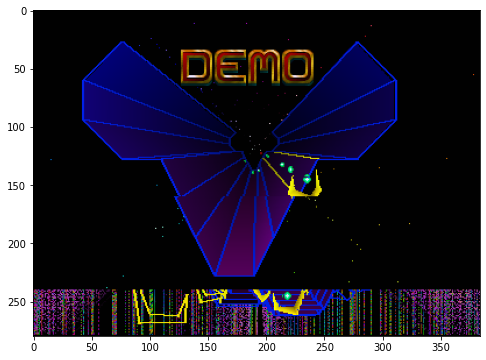
\includegraphics[height=4.2cm]{object_list/data_1.png}%
          }
        } \\
        \addlinespace
          \tcode{00,00,80,06,01,80,CF,F8}
        &
        \makecell[tl]{
          \begingroup
          \renewcommand{\arraystretch}{.8} % Default value: 1
          \begin{tabular}[t]{ll}
            \tcode{XPOS: -7   } &  \tcode{REFLECT: 0}  \\
            \tcode{DEPTH: 4} &    \tcode{RMW: 0}  \\
            \tcode{PITCH: 1} &    \tcode{TRANS: 1}  \\
            \tcode{DWIDTH: 96} &  \tcode{RELEASE: 0}  \\
            \tcode{IWIDTH: 96} &  \tcode{FIRSTPIX: 0}  \\
            \tcode{INDEX: 0} & \\
          \end{tabular}
          \endgroup
        } &
        \\
        \bottomrule
      \end{tabular}
    \end{adjustbox}
  }\caption{First Bit Mapped Object in the Object List}
\end{figure}

On PAL this field of colourful noise would be written to properly and the full game field would
extend for the whole 287 pixels of screen height. The solution when playing on an NTSC television
screen was simply to truncate the height and give the player just enough space to play the game
while missing out on activity that extended below the direct field of play.

\begin{figure}[H]
    \centering
    \begin{adjustbox}{width=11cm,center}
      \frame{
\includegraphics[width=12cm]{src/object_list/data_1_glitch.png}}%
    \end{adjustbox}
\end{figure}

